\begin{section}{Numeric results}
\label{Numerics}

\begin{subsection}{One dimensional system}

We will start with a one dimensional chain with hamiltonian $\hat{H} = \sum_{\langle i,j \rangle} |J_1| \bs{S}_i\bs{S}_j + \sum_{\langle \langle i,j \rangle \rangle} \nu_{ij}|D_2|\hat{e}_z\bs{S}_i \times \bs{S}_j$. This approximated Hamiltonian with no NNN exchange interaction is very simple, but it can describe some systems where it has even been observed $|\bs{D}_{2,ij}| > |J_{2,ij}|$ \cite{Chen2018}. In this case we can write $\bs{S}(r) = S(\cos(kr), \sin(kr), 0)$, where the real number $k$ plays the role of the wavevector, and $\theta = ka-\pi$ is the deviation from the N\'eel state. Then the classical energy per site is given by:

\begin{equation}
\frac{E(\theta)}{2S^2} = -|J_1|\cos(\theta) + |D_2|\sin(2 \theta)
\end{equation}

and the energy is minimized for $\theta^* = \arcsin(\frac{\frac{J1}{D2} - \sqrt{(\frac{J1}{D2})^2+32}}{8})$, i.e. $\theta^* = \theta^*(\frac{J1}{D2})$. Next we will show numerically that the ratio between the NN and NNN parameters, $\frac{J1}{D2}$, can be modulated by the intensity of the field, and therefore the field can be used to control the SDW wavevector. 

We will use the time average approximation \ref{MFactorApprox0} so that we can write:

\begin{align}
J_{1,ij} &= J_{1,ij}^0  \sum_{n} \frac{\mathcal{J}_n(\alpha_{ij})^2}{1+n\frac{\omega}{\text{U}}} \\
D_{2,ij} &= D_{2,ij}^0  \sum_{n} \frac{\mathcal{J}_n(\alpha_{ij})^2}{1+n\frac{\omega}{\text{U}}}
\end{align}

Where $\bs{D}_{2,ij} = \hat{e}_z D_{2,ij}$ and where $J_{1,ij}^0 = J_{1}^0 = \frac{2t_1^2}{\text{U}}$ and $D_{2,ij}^0 = -\frac{4t_2\Delta\nu_{ij}}{\text{U}}$. Since $\mathcal{J}_n(-x) = (-1)^n\mathcal{J}_n(x)$ the dependance is on $|\alpha_{ij}|$ only. Now, using \ref{Def_alpha}, for circularly polarized light we have $|\alpha_{ij}| = \frac{1}{\sqrt{2}}e|\vec{R}_{ij}| \frac{E_0}{\omega} = \frac{1}{\sqrt{2}}ea \frac{E_0}{\omega} \frac{|\vec{R}_{ij}|}{a} = \frac{|\vec{R}_{ij}|}{\sqrt{2}a} \mathcal{E}$, where $a$ is the lattice constant and $\mathcal{E} = \frac{eaE_0}{\omega}$. Now, for $J_{1,ij}$, $i$ and $j$ are NN and so we can write $|\vec{R}_{ij}|=a$, whereas for $D_{2,ij}$, $i$ and $j$ are NNN and so $|\vec{R}_{ij}|=2a$. Thus:

\begin{align}
J_{1,ij} &= J_{1} = J_{1}^0  \sum_{n} \frac{\mathcal{J}_n(\frac{1}{\sqrt{2}}\mathcal{E})^2}{1+n\frac{\omega}{\text{U}}} \\
D_{2,ij} &= D_{2,ij}^0  \sum_{n} \frac{\mathcal{J}_n(\sqrt{2}\mathcal{E})^2}{1+n\frac{\omega}{\text{U}}}
\end{align}

In each case the absolute vale is independent of $i,j$.  Now, in units $\hbar=t_1=1$ we measure energy in units of $t_1$ and frequency in units of $\frac{t_1}{\hbar}$. Then, for $t_2 = 0.1$, $\Delta = 0.5$, $\text{U} = 10$ and $\omega = 6$ we obtain \ref{Fig1:NNvsNNN}. The ratio $\frac{J_{1,ij}}{D_{2,ij}}$ is plotted in \ref{Fig1:ratio}. Finally, in \ref{Fig2} we plot the SDW NN angle $\theta$.

\begin{figure}
\centering
\begin{subfigure}{.5\textwidth}
  \centering
  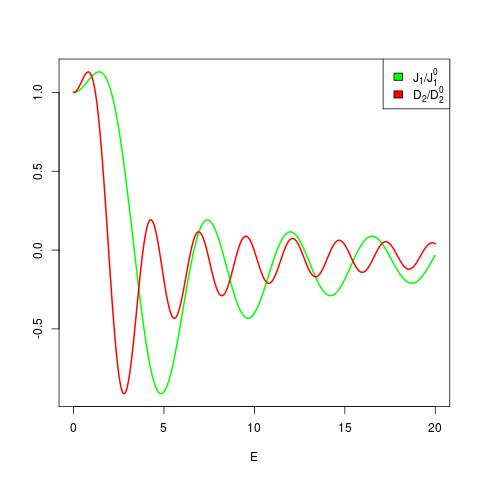
\includegraphics[width=1\linewidth]{Chapters/NNvsNNN.pdf}
  \caption{$\frac{J_{1}}{J_{1}^0}$ and $\frac{D_{2,ij}}{D_{2,ij}^0}$ are plotted as function of $\mathcal{E}$. Similar results are obtained in \cite{Mentink2015} for $J_{1}$.}
  \label{Fig1:NNvsNNN}
\end{subfigure}%
\begin{subfigure}{.5\textwidth}
  \centering
  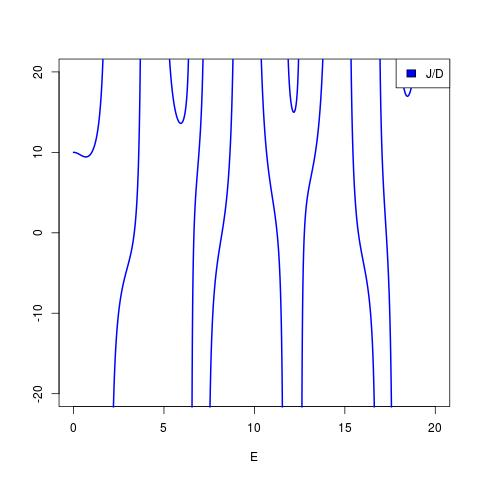
\includegraphics[width=1\linewidth]{Chapters/ratio.pdf}
  \caption{$\frac{J_{1}}{D_{2,ij}}$ is plotted as function of $\mathcal{E}$, it diverges every time $D_{2,ij}$ changes sign.}
  \label{Fig1:ratio}
\end{subfigure}
\label{Fig1}
\end{figure}

\begin{figure}
\centering
  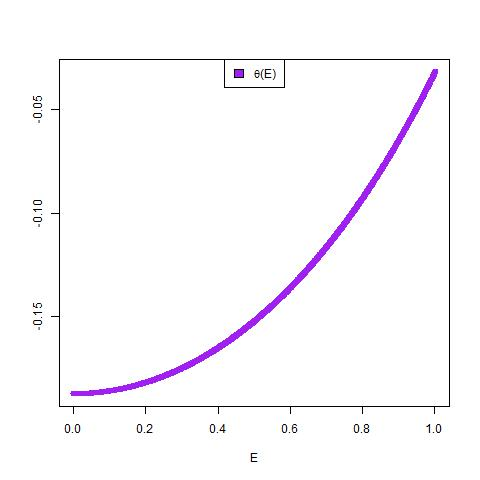
\includegraphics[width=0.5\linewidth]{Chapters/theta.pdf}
  \caption{The spin wave density NN angle $\theta$ as a function of $\mathcal{E}$. The field modifies the ratio $\frac{J_{1}}{D_{2,ij}}$ thus modifying the wave vector.}
\label{Fig2}
\end{figure}

\end{subsection}

\begin{subsection}{Two dimensional systems}
 
In a honeycomb lattice described by \ref{MKMHeff} the usual approach is 

\end{subsection}

\end{section}
